\section{XMPulldown  Class Reference}
\label{classXMPulldown}\index{XMPulldown@{XMPulldown}}
{\tt \#include $<$XMMenus.h$>$}

Inheritance diagram for XMPulldown::\begin{figure}[H]
\begin{center}
\leavevmode
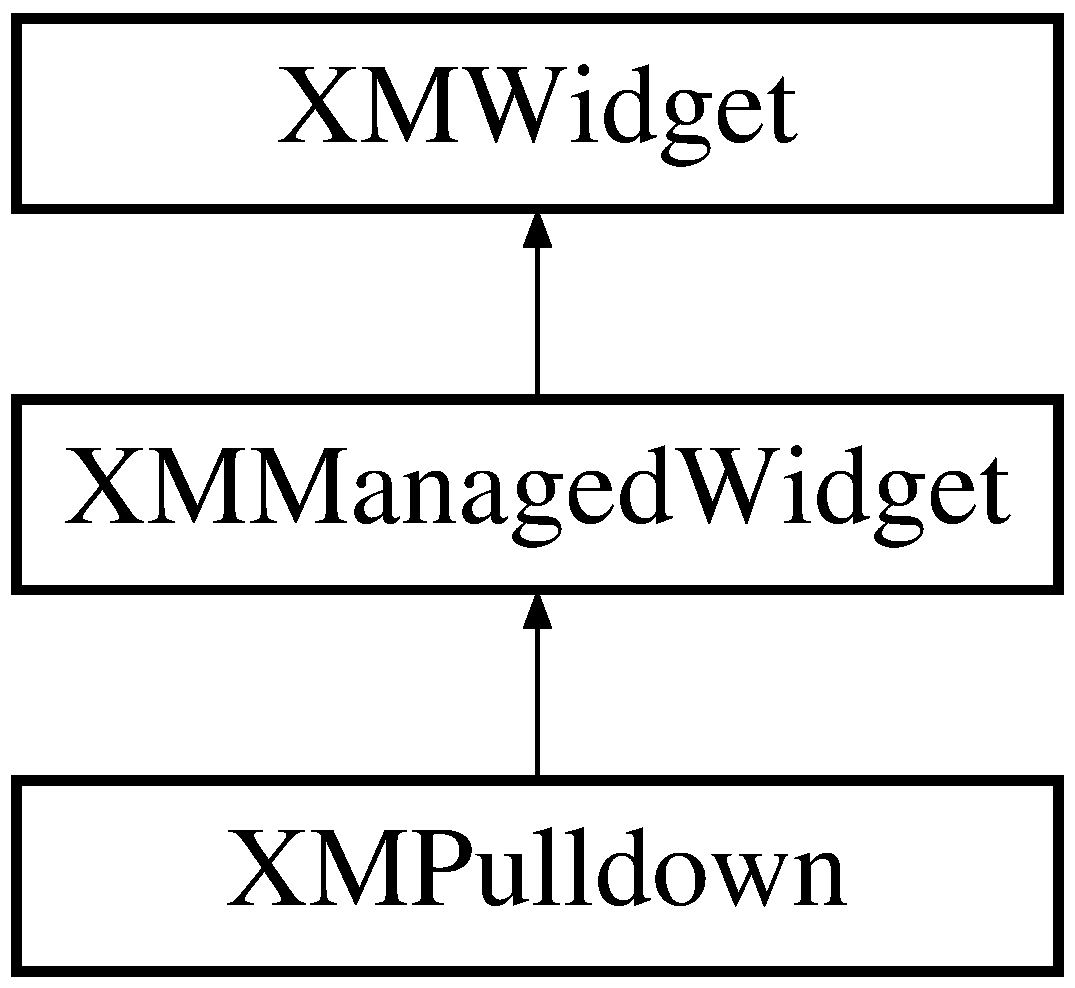
\includegraphics[height=3cm]{classXMPulldown}
\end{center}
\end{figure}
\subsection*{Public Methods}
\begin{CompactItemize}
\item 
{\bf XMPulldown} (char $\ast$n, Widget \&parent, Cardinal max\_\-items, Arg\-List l=NULL, Cardinal num\_\-args=0)
\item 
{\bf XMPulldown} (char $\ast$n, {\bf XMWidget} \&parent, Cardinal max\_\-items, Arg\-List l=NULL, Cardinal num\_\-args=0)
\item 
{\bf $\sim$XMPulldown} ()
\item 
void {\bf Label} (char $\ast$label)
\item 
void {\bf Radio\-Menu} ()
\item 
void {\bf Radio\-Force\-One} ()
\item 
void {\bf No\-Radio\-Menu} ()
\item 
void {\bf Radio\-No\-Force\-One} ()
\item 
{\bf XMPush\-Button} $\ast$ {\bf Add\-Menu\-Button} (char $\ast$n, void($\ast$callback)({\bf XMWidget} $\ast$, Xt\-Pointer, Xt\-Pointer)=NULL, Xt\-Pointer client\_\-data=NULL, Arg\-List l=NULL, Cardinal num\_\-args=0)
\item 
{\bf XMToggle\-Button} $\ast$ {\bf Add\-Menu\-Toggle\-Button} (char $\ast$n, void($\ast$callback)({\bf XMWidget} $\ast$, Xt\-Pointer, Xt\-Pointer)=NULL, Xt\-Pointer client\_\-data=NULL, Arg\-List l=NULL, Cardinal num\_\-args=0)
\item 
{\bf XMWidget} $\ast$ {\bf Add\-Separator} ()
\item 
XMPulldown $\ast$ {\bf Add\-Submenu} (char $\ast$n, int max\_\-items, Arg\-List l=NULL, Cardinal num\_\-args=0)
\item 
int {\bf Menu\-Size} ()
\item 
int {\bf Max\-Menu\-Size} ()
\item 
{\bf XMMenu\-Item} $\ast$ {\bf Get\-Menu\-Item} (Cardinal index)
\item 
{\bf XMMenu\-Item} $\ast$ {\bf Find\-Menu\-Item} (char $\ast$n)
\item 
{\bf XMWidget} $\ast$ {\bf Get\-Cascade\-Button} ()
\item 
{\bf XMMenu\-Item} $\ast$ {\bf Get\-Next\-Menu\-Item} ()
\item 
{\bf XMMenu\-Item} $\ast$ {\bf Get\-First\-Menu\-Item} ()
\end{CompactItemize}
\subsection*{Protected Methods}
\begin{CompactItemize}
\item 
void {\bf Build\-Menu} (Cardinal max\_\-items, Widget parent, Arg\-List l, Cardinal num\_\-args)
\end{CompactItemize}
\subsection*{Protected Attributes}
\begin{CompactItemize}
\item 
{\bf XMCascade\-Button} $\ast$ {\bf pd\_\-button}
\item 
{\bf XMMenu\-Item} $\ast$ {\bf menu\_\-items}
\item 
Cardinal {\bf menu\_\-count}
\item 
Cardinal {\bf max\_\-menu\_\-items}
\item 
Cardinal {\bf menu\_\-cursor}
\end{CompactItemize}


\subsection{Constructor \& Destructor Documentation}
\index{XMPulldown@{XMPulldown}!XMPulldown@{XMPulldown}}
\index{XMPulldown@{XMPulldown}!XMPulldown@{XMPulldown}}
\subsubsection{\setlength{\rightskip}{0pt plus 5cm}XMPulldown::XMPulldown (char $\ast$ {\em n}, Widget \& {\em parent}, Cardinal {\em max\_\-items}, Arg\-List {\em l} = NULL, Cardinal {\em num\_\-args} = 0)\hspace{0.3cm}{\tt  [inline]}}\label{classXMPulldown_a0}




Definition at line 329 of file XMMenus.h.

References Build\-Menu().

Referenced by Add\-Submenu().\index{XMPulldown@{XMPulldown}!XMPulldown@{XMPulldown}}
\index{XMPulldown@{XMPulldown}!XMPulldown@{XMPulldown}}
\subsubsection{\setlength{\rightskip}{0pt plus 5cm}XMPulldown::XMPulldown (char $\ast$ {\em n}, {\bf XMWidget} \& {\em parent}, Cardinal {\em max\_\-items}, Arg\-List {\em l} = NULL, Cardinal {\em num\_\-args} = 0)\hspace{0.3cm}{\tt  [inline]}}\label{classXMPulldown_a1}




Definition at line 335 of file XMMenus.h.

References Build\-Menu(), and XMWidget::getid().\index{XMPulldown@{XMPulldown}!~XMPulldown@{$\sim$XMPulldown}}
\index{~XMPulldown@{$\sim$XMPulldown}!XMPulldown@{XMPulldown}}
\subsubsection{\setlength{\rightskip}{0pt plus 5cm}XMPulldown::$\sim$XMPulldown ()}\label{classXMPulldown_a2}




Definition at line 379 of file XMMenus.cpp.

References Button, XMMenu\-Item::item, menu\_\-count, menu\_\-items, pd\_\-button, Separator, Submenu, Toggle\-Button, XMMenu\-Item::type, and Unused.

\subsection{Member Function Documentation}
\index{XMPulldown@{XMPulldown}!AddMenuButton@{AddMenuButton}}
\index{AddMenuButton@{AddMenuButton}!XMPulldown@{XMPulldown}}
\subsubsection{\setlength{\rightskip}{0pt plus 5cm}{\bf XMPush\-Button} $\ast$ XMPulldown::Add\-Menu\-Button (char $\ast$ {\em n}, void($\ast$ {\em callback})({\bf XMWidget} $\ast$, Xt\-Pointer, Xt\-Pointer) = NULL, Xt\-Pointer {\em client\_\-data} = NULL, Arg\-List {\em l} = NULL, Cardinal {\em num\_\-args} = 0)}\label{classXMPulldown_a8}




Definition at line 442 of file XMMenus.cpp.

References Button, exit(), max\_\-menu\_\-items, menu\_\-count, menu\_\-items, XMWidget::name, and XMWidget::Set\-Attribute().\index{XMPulldown@{XMPulldown}!AddMenuToggleButton@{AddMenuToggleButton}}
\index{AddMenuToggleButton@{AddMenuToggleButton}!XMPulldown@{XMPulldown}}
\subsubsection{\setlength{\rightskip}{0pt plus 5cm}{\bf XMToggle\-Button} $\ast$ XMPulldown::Add\-Menu\-Toggle\-Button (char $\ast$ {\em n}, void($\ast$ {\em callback})({\bf XMWidget} $\ast$, Xt\-Pointer, Xt\-Pointer) = NULL, Xt\-Pointer {\em client\_\-data} = NULL, Arg\-List {\em l} = NULL, Cardinal {\em num\_\-args} = 0)}\label{classXMPulldown_a9}




Definition at line 500 of file XMMenus.cpp.

References exit(), max\_\-menu\_\-items, menu\_\-count, menu\_\-items, XMWidget::name, XMWidget::Set\-Attribute(), and Toggle\-Button.\index{XMPulldown@{XMPulldown}!AddSeparator@{AddSeparator}}
\index{AddSeparator@{AddSeparator}!XMPulldown@{XMPulldown}}
\subsubsection{\setlength{\rightskip}{0pt plus 5cm}{\bf XMWidget} $\ast$ XMPulldown::Add\-Separator ()}\label{classXMPulldown_a10}




Definition at line 548 of file XMMenus.cpp.

References exit(), max\_\-menu\_\-items, menu\_\-count, menu\_\-items, Separator, and XMManaged\-Widget::XMManaged\-Widget().\index{XMPulldown@{XMPulldown}!AddSubmenu@{AddSubmenu}}
\index{AddSubmenu@{AddSubmenu}!XMPulldown@{XMPulldown}}
\subsubsection{\setlength{\rightskip}{0pt plus 5cm}XMPulldown $\ast$ XMPulldown::Add\-Submenu (char $\ast$ {\em n}, int {\em max\_\-items}, Arg\-List {\em l} = NULL, Cardinal {\em num\_\-args} = 0)}\label{classXMPulldown_a11}




Definition at line 600 of file XMMenus.cpp.

References exit(), max\_\-menu\_\-items, menu\_\-count, menu\_\-items, Submenu, and XMPulldown().\index{XMPulldown@{XMPulldown}!BuildMenu@{BuildMenu}}
\index{BuildMenu@{BuildMenu}!XMPulldown@{XMPulldown}}
\subsubsection{\setlength{\rightskip}{0pt plus 5cm}void XMPulldown::Build\-Menu (Cardinal {\em max\_\-items}, Widget {\em parent}, Arg\-List {\em l}, Cardinal {\em num\_\-args})\hspace{0.3cm}{\tt  [protected]}}\label{classXMPulldown_b0}




Definition at line 332 of file XMMenus.cpp.

References exit(), XMWidget::id, XMMenu\-Item::item, XMButton::Label(), max\_\-menu\_\-items, menu\_\-count, menu\_\-items, XMWidget::name, pd\_\-button, XMCascade\-Button::Set\-Associated\-Menu(), XMButton::Set\-Mnemonic(), XMMenu\-Item::type, and Unused.

Referenced by XMPulldown().\index{XMPulldown@{XMPulldown}!FindMenuItem@{FindMenuItem}}
\index{FindMenuItem@{FindMenuItem}!XMPulldown@{XMPulldown}}
\subsubsection{\setlength{\rightskip}{0pt plus 5cm}{\bf XMMenu\-Item} $\ast$ XMPulldown::Find\-Menu\-Item (char $\ast$ {\em n})}\label{classXMPulldown_a15}




Definition at line 641 of file XMMenus.cpp.

References Button, exit(), XMWidget::getname(), XMMenu\-Item::item, menu\_\-count, menu\_\-items, Separator, Submenu, Toggle\-Button, XMMenu\-Item::type, and Unused.

Referenced by XMMenu\-Bar::Get\-Menu\-Item().\index{XMPulldown@{XMPulldown}!GetCascadeButton@{GetCascadeButton}}
\index{GetCascadeButton@{GetCascadeButton}!XMPulldown@{XMPulldown}}
\subsubsection{\setlength{\rightskip}{0pt plus 5cm}{\bf XMWidget}$\ast$ XMPulldown::Get\-Cascade\-Button ()\hspace{0.3cm}{\tt  [inline]}}\label{classXMPulldown_a16}




Definition at line 394 of file XMMenus.h.

Referenced by XMMenu\-Bar::Add\-Help\-Pulldown().\index{XMPulldown@{XMPulldown}!GetFirstMenuItem@{GetFirstMenuItem}}
\index{GetFirstMenuItem@{GetFirstMenuItem}!XMPulldown@{XMPulldown}}
\subsubsection{\setlength{\rightskip}{0pt plus 5cm}{\bf XMMenu\-Item}$\ast$ XMPulldown::Get\-First\-Menu\-Item ()\hspace{0.3cm}{\tt  [inline]}}\label{classXMPulldown_a18}




Definition at line 400 of file XMMenus.h.

References Get\-Next\-Menu\-Item(), and menu\_\-cursor.\index{XMPulldown@{XMPulldown}!GetMenuItem@{GetMenuItem}}
\index{GetMenuItem@{GetMenuItem}!XMPulldown@{XMPulldown}}
\subsubsection{\setlength{\rightskip}{0pt plus 5cm}{\bf XMMenu\-Item}$\ast$ XMPulldown::Get\-Menu\-Item (Cardinal {\em index})\hspace{0.3cm}{\tt  [inline]}}\label{classXMPulldown_a14}




Definition at line 390 of file XMMenus.h.

References menu\_\-count.\index{XMPulldown@{XMPulldown}!GetNextMenuItem@{GetNextMenuItem}}
\index{GetNextMenuItem@{GetNextMenuItem}!XMPulldown@{XMPulldown}}
\subsubsection{\setlength{\rightskip}{0pt plus 5cm}{\bf XMMenu\-Item} $\ast$ XMPulldown::Get\-Next\-Menu\-Item ()}\label{classXMPulldown_a17}




Definition at line 680 of file XMMenus.cpp.

References menu\_\-count, menu\_\-cursor, and menu\_\-items.

Referenced by Get\-First\-Menu\-Item().\index{XMPulldown@{XMPulldown}!Label@{Label}}
\index{Label@{Label}!XMPulldown@{XMPulldown}}
\subsubsection{\setlength{\rightskip}{0pt plus 5cm}void XMPulldown::Label (char $\ast$ {\em label})\hspace{0.3cm}{\tt  [inline]}}\label{classXMPulldown_a3}




Definition at line 345 of file XMMenus.h.

References XMButton::Label().\index{XMPulldown@{XMPulldown}!MaxMenuSize@{MaxMenuSize}}
\index{MaxMenuSize@{MaxMenuSize}!XMPulldown@{XMPulldown}}
\subsubsection{\setlength{\rightskip}{0pt plus 5cm}int XMPulldown::Max\-Menu\-Size ()\hspace{0.3cm}{\tt  [inline]}}\label{classXMPulldown_a13}




Definition at line 389 of file XMMenus.h.

References max\_\-menu\_\-items.\index{XMPulldown@{XMPulldown}!MenuSize@{MenuSize}}
\index{MenuSize@{MenuSize}!XMPulldown@{XMPulldown}}
\subsubsection{\setlength{\rightskip}{0pt plus 5cm}int XMPulldown::Menu\-Size ()\hspace{0.3cm}{\tt  [inline]}}\label{classXMPulldown_a12}




Definition at line 388 of file XMMenus.h.

References menu\_\-count.\index{XMPulldown@{XMPulldown}!NoRadioMenu@{NoRadioMenu}}
\index{NoRadioMenu@{NoRadioMenu}!XMPulldown@{XMPulldown}}
\subsubsection{\setlength{\rightskip}{0pt plus 5cm}void XMPulldown::No\-Radio\-Menu ()\hspace{0.3cm}{\tt  [inline]}}\label{classXMPulldown_a6}




Definition at line 355 of file XMMenus.h.

References XMWidget::Set\-Attribute().\index{XMPulldown@{XMPulldown}!RadioForceOne@{RadioForceOne}}
\index{RadioForceOne@{RadioForceOne}!XMPulldown@{XMPulldown}}
\subsubsection{\setlength{\rightskip}{0pt plus 5cm}void XMPulldown::Radio\-Force\-One ()\hspace{0.3cm}{\tt  [inline]}}\label{classXMPulldown_a5}




Definition at line 351 of file XMMenus.h.

References XMWidget::Set\-Attribute().\index{XMPulldown@{XMPulldown}!RadioMenu@{RadioMenu}}
\index{RadioMenu@{RadioMenu}!XMPulldown@{XMPulldown}}
\subsubsection{\setlength{\rightskip}{0pt plus 5cm}void XMPulldown::Radio\-Menu ()\hspace{0.3cm}{\tt  [inline]}}\label{classXMPulldown_a4}




Definition at line 349 of file XMMenus.h.

References XMWidget::Set\-Attribute().\index{XMPulldown@{XMPulldown}!RadioNoForceOne@{RadioNoForceOne}}
\index{RadioNoForceOne@{RadioNoForceOne}!XMPulldown@{XMPulldown}}
\subsubsection{\setlength{\rightskip}{0pt plus 5cm}void XMPulldown::Radio\-No\-Force\-One ()\hspace{0.3cm}{\tt  [inline]}}\label{classXMPulldown_a7}




Definition at line 357 of file XMMenus.h.

References XMWidget::Set\-Attribute().

\subsection{Member Data Documentation}
\index{XMPulldown@{XMPulldown}!max_menu_items@{max\_\-menu\_\-items}}
\index{max_menu_items@{max\_\-menu\_\-items}!XMPulldown@{XMPulldown}}
\subsubsection{\setlength{\rightskip}{0pt plus 5cm}Cardinal XMPulldown::max\_\-menu\_\-items\hspace{0.3cm}{\tt  [protected]}}\label{classXMPulldown_n3}




Definition at line 322 of file XMMenus.h.

Referenced by Add\-Menu\-Button(), Add\-Menu\-Toggle\-Button(), Add\-Separator(), Add\-Submenu(), Build\-Menu(), and Max\-Menu\-Size().\index{XMPulldown@{XMPulldown}!menu_count@{menu\_\-count}}
\index{menu_count@{menu\_\-count}!XMPulldown@{XMPulldown}}
\subsubsection{\setlength{\rightskip}{0pt plus 5cm}Cardinal XMPulldown::menu\_\-count\hspace{0.3cm}{\tt  [protected]}}\label{classXMPulldown_n2}




Definition at line 321 of file XMMenus.h.

Referenced by Add\-Menu\-Button(), Add\-Menu\-Toggle\-Button(), Add\-Separator(), Add\-Submenu(), Build\-Menu(), Find\-Menu\-Item(), Get\-Menu\-Item(), Get\-Next\-Menu\-Item(), Menu\-Size(), and $\sim$XMPulldown().\index{XMPulldown@{XMPulldown}!menu_cursor@{menu\_\-cursor}}
\index{menu_cursor@{menu\_\-cursor}!XMPulldown@{XMPulldown}}
\subsubsection{\setlength{\rightskip}{0pt plus 5cm}Cardinal XMPulldown::menu\_\-cursor\hspace{0.3cm}{\tt  [protected]}}\label{classXMPulldown_n4}




Definition at line 323 of file XMMenus.h.

Referenced by Get\-First\-Menu\-Item(), and Get\-Next\-Menu\-Item().\index{XMPulldown@{XMPulldown}!menu_items@{menu\_\-items}}
\index{menu_items@{menu\_\-items}!XMPulldown@{XMPulldown}}
\subsubsection{\setlength{\rightskip}{0pt plus 5cm}{\bf XMMenu\-Item}$\ast$ XMPulldown::menu\_\-items\hspace{0.3cm}{\tt  [protected]}}\label{classXMPulldown_n1}




Definition at line 320 of file XMMenus.h.

Referenced by Add\-Menu\-Button(), Add\-Menu\-Toggle\-Button(), Add\-Separator(), Add\-Submenu(), Build\-Menu(), Find\-Menu\-Item(), Get\-Next\-Menu\-Item(), and $\sim$XMPulldown().\index{XMPulldown@{XMPulldown}!pd_button@{pd\_\-button}}
\index{pd_button@{pd\_\-button}!XMPulldown@{XMPulldown}}
\subsubsection{\setlength{\rightskip}{0pt plus 5cm}{\bf XMCascade\-Button}$\ast$ XMPulldown::pd\_\-button\hspace{0.3cm}{\tt  [protected]}}\label{classXMPulldown_n0}




Definition at line 319 of file XMMenus.h.

Referenced by Build\-Menu(), and $\sim$XMPulldown().

The documentation for this class was generated from the following files:\begin{CompactItemize}
\item 
{\bf XMMenus.h}\item 
{\bf XMMenus.cpp}\end{CompactItemize}
